\documentclass[11pt,a4paper]{article}

\usepackage[margin=1in]{geometry}
\usepackage[T1]{fontenc}
\usepackage[utf8]{inputenc}
\usepackage{lmodern}
\usepackage{microtype}
\usepackage{setspace}
\usepackage{amsmath,amssymb}
\usepackage{booktabs}
\usepackage{hyperref}
\usepackage[dvipsnames]{xcolor}
\usepackage{tikz}
\usetikzlibrary{arrows.meta,positioning,shapes.geometric,fit,backgrounds}

\hypersetup{
  colorlinks=true,
  linkcolor=MidnightBlue,
  urlcolor=RoyalBlue,
  citecolor=MidnightBlue
}

\setstretch{1.1}
\setlength{\parskip}{0.4em}
\setlength{\parindent}{0pt}

\title{NeuroMotion: End-to-End Notes\\\large From Movement to Synthetic EMG}
\author{Project Notes}
\date{\today}

\begin{document}
\maketitle

\section{What this repository does}

\textbf{Goal:} generate realistic multi-channel synthetic EMG from a planned hand/wrist movement.

The repository links four pieces:
\begin{enumerate}
    \item Musculoskeletal simulation (OpenSim model, joint kinematics, muscle lengths)
    \item Motor neuron pool physiology (recruitment and spike trains)
    \item MUAP waveform generation (BioMime model)
    \item Signal composition (sum MU contributions across channels over time)
\end{enumerate}

\section{Main folders and their role}

\begin{tabular}{@{}ll@{}}
\toprule
\textbf{Path} & \textbf{Purpose} \\
\midrule
\texttt{NeuroMotion/MSKlib} & OpenSim movement + muscle-parameter extraction \\
\texttt{NeuroMotion/MNPoollib} & Motor neuron pool model + spike train generation \\
\texttt{NeuroMotion/EMGSyn.py} & EMG synthesis logic and orchestration \\
\texttt{scripts/mov2emg.py} & End-to-end runnable pipeline \\
\texttt{ckp/} & Config and pretrained weights (BioMime model) \\
\bottomrule
\end{tabular}

\section{What is the \texttt{.osim} model and why it matters}

\subsection*{What \texttt{.osim} is}
A \texttt{.osim} file is the OpenSim model definition: bones, joints, constraints, muscles, tendon paths, and mechanical properties.

\subsection*{Why it is needed here}
Without \texttt{.osim}, movement is only a list of angles. With \texttt{.osim}, the code can compute muscle-specific biomechanical changes over time, for example fiber length trajectories. Those trajectories condition neural and MUAP behavior, improving physiological realism.

\subsection*{Difference between \texttt{.osim} and \texttt{.mot}}
\begin{itemize}
    \item \texttt{.osim}: model specification (anatomy and mechanics)
    \item \texttt{.mot}: time-series motion (joint coordinates over time)
\end{itemize}

\section{Pipeline from beginning to end}

\subsection*{Step 1 --- Define movement trajectory}
In \texttt{scripts/mov2emg.py}, a movement sequence is defined as poses and durations.
This is converted into a smooth joint-angle trajectory sampled in time.

\subsection*{Step 2 --- Run OpenSim and extract muscle changes}
\texttt{MSKModel} applies each joint state to the OpenSim model and computes muscle lengths.
Then \texttt{len2params()} derives parameter changes (e.g., depth/CV/length trends) used downstream.

\subsection*{Step 3 --- Simulate motor neuron pool activity}
For a target muscle (e.g., FDSI), \texttt{MotoneuronPool} initializes motor units and produces spike trains from neural drive/excitation.

\subsection*{Step 4 --- Generate dynamic MUAPs (BioMime)}
The generator model takes physiological conditioning variables and produces MUAP waveforms per motor unit and per time step.

\subsection*{Step 5 --- Compose final EMG signal}
EMG channels are synthesized by summing all active MU contributions at spike times.
The script saves figures (spikes, MUAP snapshots, EMG image) and output arrays.

\section{Visual overview}

\begin{center}
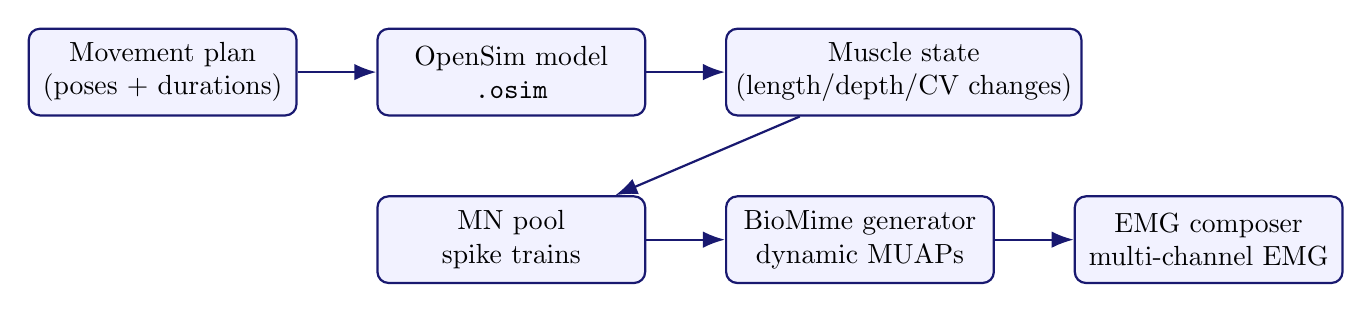
\begin{tikzpicture}[
    node distance=10mm and 10mm,
    block/.style={rectangle, rounded corners, draw=MidnightBlue, thick, align=center, minimum width=3.4cm, minimum height=1.1cm, fill=blue!5},
    arrow/.style={-{Latex[length=2.8mm]}, thick, draw=MidnightBlue}
]

\node[block] (a) {Movement plan\\(poses + durations)};
\node[block, right=of a] (b) {OpenSim model\\\texttt{.osim}};
\node[block, right=of b] (c) {Muscle state\\(length/depth/CV changes)};
\node[block, below=of b] (d) {MN pool\\spike trains};
\node[block, right=of d] (e) {BioMime generator\\dynamic MUAPs};
\node[block, right=of e] (f) {EMG composer\\multi-channel EMG};

\draw[arrow] (a) -- (b);
\draw[arrow] (b) -- (c);
\draw[arrow] (c) -- (d);
\draw[arrow] (d) -- (e);
\draw[arrow] (e) -- (f);

\end{tikzpicture}
\end{center}

\section{How EMG is generated (mathematical view)}

For each channel $c$, synthetic EMG is formed by superposition:
\[
\mathrm{EMG}_c(t) = \sum_{m=1}^{N_{MU}}\ \sum_{k\in\mathcal{S}_m} \mathrm{MUAP}_{c,m}(t-t_k) + n_c(t)
\]
where:
\begin{itemize}
    \item $\mathcal{S}_m$ = spike times of motor unit $m$
    \item $\mathrm{MUAP}_{c,m}(\cdot)$ = channel-specific waveform for unit $m$
    \item $n_c(t)$ = optional noise/perturbation term
\end{itemize}

\section{Practical run path in this repo}

\begin{itemize}
    \item Main run script: \texttt{scripts/mov2emg.py}
    \item Movement visualization utility: \texttt{scripts/visualize\_movement.py}
    \item OpenSim movement export: \texttt{MSKModel.write\_mov(...)} creates \texttt{.mot}
\end{itemize}

Typical generated outputs include:
\begin{itemize}
    \item \texttt{figs/spikes\_*.jpg}
    \item \texttt{res/emg\_*.jpg}
    \item \texttt{res/*muap*.jpg}
    \item \texttt{vis\_output/movement.mot}
\end{itemize}

\section{Why this pipeline is useful}

\begin{itemize}
    \item Create labeled EMG data without repeated human data collection
    \item Stress-test decomposition and gesture-recognition algorithms
    \item Study parameter effects (recruitment, MUAP morphology, movement dynamics)
    \item Prototype quickly before wet-lab/hardware experiments
\end{itemize}

\section{Quick compile command}

From repository root:
\begin{verbatim}
pdflatex -output-directory notes notes/neuromotion_notes.tex
\end{verbatim}

If \texttt{pdflatex} is not installed:
\begin{verbatim}
sudo apt update
sudo apt install -y texlive-latex-extra texlive-fonts-recommended
\end{verbatim}

\end{document}
